\begin{enumerate}[label=\arabic*.,ref=\theenumi]
%\begin{enumerate}[label=\thesubsection.\arabic*.,ref=\thesubsection.\theenumi]

\item  There is a button adjacent to the USB port of the pico.  
Keep this button (BOOTSEL) pressed while connecting the 
RPi to the Pico through the USB cable.
\item Login to termux-debian and execute the following commands.
\begin{lstlisting}
cd pico/trunk/arm/codes/setup/blink
mkdir build #Only once
cd build
cmake ..
make -j4
scp  main.uf2 pi@192.168.0.114:
\end{lstlisting}
Suitably modify the above ip address before sending main.uf2 .
\item Now login to the raspberry pi and execute the following commands.
\begin{lstlisting}
sudo mkdir /mnt/pico #Only once
sudo fdisk -l
sudo mount /dev/sda1 /mnt/pico
sudo mv /mnt/pico
sudo umount /mnt/pico
\end{lstlisting}
You should now see the LED to the right of the USB port blinking.
\item Connect RUN on pico to GND.  Keep pressing BOOTSEL while removing
the RUN-GND wire from GND.  The LED stops blinking.  Pico is now ready to be flashed.
\end{enumerate}
%
\subsection{Delay}
\begin{enumerate}[label=\arabic*.,ref=\theenumi]
%\begin{enumerate}[label=\thesubsection.\arabic*.,ref=\thesubsection.\theenumi]
\item Note the followign lines in the C code below:
\begin{lstlisting}
codes/setup/blink/main.c
\end{lstlisting}
%
\begin{lstlisting}
	gpio_put(LED_PIN, 1);
        sleep_ms(250);
        gpio_put(LED_PIN, 0);
        sleep_ms(250);
\end{lstlisting}
%
It is obvious that the blink period is 500ms = 0.5s
\item Replace the below instruction in the C program
\begin{lstlisting}
        sleep_ms(250);
\end{lstlisting}
%
with
\begin{lstlisting}
        sleep_ms(500);
\end{lstlisting}
Can you see any difference in the LED blinking frequency?

\item Now modify the above code to keep the LED on permanently.
\\
\solution Execute the following code.
\begin{lstlisting}
pico/codes/setup/onoff/main.c
\end{lstlisting}
\item Use GP2 as an output pin and drive an LED.
\\
\solution  Connect the LED to pico as per Table \ref{table:setup_led} and Fig. \ref{fig:pin_sheet}

\begin{lstlisting}
pico/codes/setup/gpio/main.c
\end{lstlisting}

\begin{table}[!ht]
\centering
\begin{tabular}{|l|l|l|}
\hline
Type & pico  pin  &  Destination \\ \hline
Output &  3V3 &  LED\\ \hline
Output  & GP2  &  LED\\ \hline
\end{tabular}
\caption{Connection between LED and pico}
\label{table:setup_led}
\end{table}

\item  Execute the following code.  Connect a wire to GND and touch GP2 on the pico.  The onboard LED will turn off.
Repeat this exercise to blink the LED manually.
\begin{lstlisting}
pico/codes/setup/input/main.c
\end{lstlisting}


\begin{figure}[!ht]
\centering
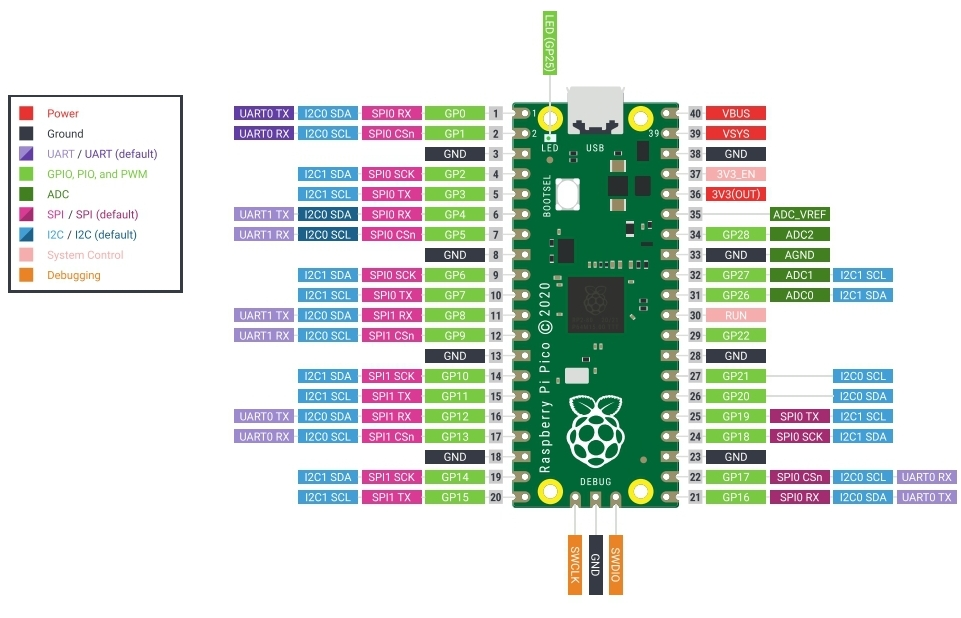
\includegraphics[width = \columnwidth]{pico/arm/setup/figs/pin_sheet.jpg}
\caption{Pin diagram}
\label{fig:pin_sheet}
\end{figure}
\item Execute the following code to drive the seven segment display.
\begin{lstlisting}
pico/arm/codes/sevenseg/static/main.c
\end{lstlisting}
\end{enumerate}



